% This is "sig-alternate.tex" V2.0 May 2012
% This file should be compiled with V2.5 of "sig-alternate.cls" May 2012
%
% This example file demonstrates the use of the 'sig-alternate.cls'
% V2.5 LaTeX2e document class file. It is for those submitting
% articles to ACM Conference Proceedings WHO DO NOT WISH TO
% STRICTLY ADHERE TO THE SIGS (PUBS-BOARD-ENDORSED) STYLE.
% The 'sig-alternate.cls' file will produce a similar-looking,
% albeit, 'tighter' paper resulting in, invariably, fewer pages.
%
% ----------------------------------------------------------------------------------------------------------------
% This .tex file (and associated .cls V2.5) produces:
%       1) The Permission Statement
%       2) The Conference (location) Info information
%       3) The Copyright Line with ACM data
%       4) NO page numbers
%
% as against the acm_proc_article-sp.cls file which
% DOES NOT produce 1) thru' 3) above.
%
% Using 'sig-alternate.cls' you have control, however, from within
% the source .tex file, over both the CopyrightYear
% (defaulted to 200X) and the ACM Copyright Data
% (defaulted to X-XXXXX-XX-X/XX/XX).
% e.g.
% \CopyrightYear{2007} will cause 2007 to appear in the copyright line.
% \crdata{0-12345-67-8/90/12} will cause 0-12345-67-8/90/12 to appear in the copyright line.
%
% ---------------------------------------------------------------------------------------------------------------
% This .tex source is an example which *does* use
% the .bib file (from which the .bbl file % is produced).
% REMEMBER HOWEVER: After having produced the .bbl file,
% and prior to final submission, you *NEED* to 'insert'
% your .bbl file into your source .tex file so as to provide
% ONE 'self-contained' source file.
%
% ================= IF YOU HAVE QUESTIONS =======================
% Questions regarding the SIGS styles, SIGS policies and
% procedures, Conferences etc. should be sent to
% Adrienne Griscti (griscti@acm.org)
%
% Technical questions _only_ to
% Gerald Murray (murray@hq.acm.org)
% ===============================================================
%
% For tracking purposes - this is V2.0 - May 2012

\documentclass{sig-alternate}
\usepackage{placeins}
\usepackage{verbatim}
\usepackage{graphicx}
\usepackage{epstopdf}
\usepackage{subfigure}

\begin{document}
%
% --- Author Metadata here ---
\conferenceinfo{SIGIR}{'15, August 9-13, 2015, Santiago, Chile}
%\CopyrightYear{2007} % Allows default copyright year (20XX) to be over-ridden - IF NEED BE.
%\crdata{0-12345-67-8/90/01}  % Allows default copyright data (0-89791-88-6/97/05) to be over-ridden - IF NEED BE.
% --- End of Author Metadata ---

\title{On Term Selection Techniques for Patent Prior Art Search
%\titlenote{(Produces the permission block, and
%copyright information). For use with
%SIG-ALTERNATE.CLS. Supported by ACM.}
}
%\subtitle{Why Patent Prior-art Search Fails?
%\titlenote{A full version of this paper is available as
%\textit{Author's Guide to Preparing ACM SIG Proceedings Using
%\LaTeX$2_\epsilon$\ and BibTeX} at
%\texttt{www.acm.org/eaddress.htm}}
%}
%
% You need the command \numberofauthors to handle the 'placement
% and alignment' of the authors beneath the title.
%
% For aesthetic reasons, we recommend 'three authors at a time'
% i.e. three 'name/affiliation blocks' be placed beneath the title.
%
% NOTE: You are NOT restricted in how many 'rows' of
% "name/affiliations" may appear. We just ask that you restrict
% the number of 'columns' to three.
%
% Because of the available 'opening page real-estate'
% we ask you to refrain from putting more than six authors
% (two rows with three columns) beneath the article title.
% More than six makes the first-page appear very cluttered indeed.
%
% Use the \alignauthor commands to handle the names
% and affiliations for an 'aesthetic maximum' of six authors.
% Add names, affiliations, addresses for
% the seventh etc. author(s) as the argument for the
% \additionalauthors command.
% These 'additional authors' will be output/set for you
% without further effort on your part as the last section in
% the body of your article BEFORE References or any Appendices.

%\numberofauthors{3} %  in this sample file, there are a *total*
% of EIGHT authors. SIX appear on the 'first-page' (for formatting
% reasons) and the remaining two appear in the \additionalauthors section.
%
\numberofauthors{1}
\author{
%Contribution ID: 5
\alignauthor
Mona  Golestan Far$^{\dag}$, Scott Sanner$^{\ddag}$\titlenote{This work has been primarily completed while the author was at NICTA, Canberra, Australia.},  Reda Bouadjenek$^\S$, \\Gabriela Ferraro$^{\dag}$, David Hawking$^\partial$\\
$^{\dag}$\affaddr{NICTA, Australian National University,  \{mona.golestanfar, gabriela.ferraro\}@nicta.com.au}\\
$^{\ddag}$\affaddr{Oregon State University, Corvallis, OR 97331 USA, scott.sanner@oregonstate.edu}\\
$^\S$\affaddr{INRIA \& LIRMM University of Montpellier France, reda.bouadjenek@inria.fr}\\
$^\partial$\affaddr{BING Research \& Australian National University, david.hawking@acm.org}\\
}

% There's nothing stopping you putting the seventh, eighth, etc.
% author on the opening page (as the 'third row') but we ask,
% for aesthetic reasons that you place these 'additional authors'
% in the \additional authors block, viz.
%\additionalauthors{Additional authors: John Smith (The Th{\o}rv{\"a}ld Group,
%email: {\texttt{jsmith@affiliation.org}}) and Julius P.~Kumquat
%(The Kumquat Consortium, email: {\texttt{jpkumquat@consortium.net}}).}
\date{16 February 2015}
% Just remember to make sure that the TOTAL number of authors
% is the number that will appear on the first page PLUS the
% number that will appear in the \additionalauthors section.

\maketitle
\begin{abstract}
In this paper, we investigate the influence of term selection on retrieval
performance on the CLEF-IP prior Art test collection, using the Description section of the patent query with Language Model (LM) and BM25 scoring functions. We find that an oracular relevance feedback system that extracts terms from the judged relevant documents far
outperforms the baseline and performs twice as well on MAP as the best
competitor in CLEF-IP 2010.  We find a very clear term selection value
threshold for use when choosing terms.  We also noticed that most of
the useful feedback terms are actually present in the original query
and hypothesized that the baseline system could be substantially
improved by removing negative query terms.
%Furthermore, a similar oracular query restricted
%to select terms from only the reference patent performs nearly as well
%as unrestricted term selection suggesting that query reduction methods
%should suffice for state-of-the-art performance on CLEF-IP 2010.
We tried four simple automated approaches to identify negative terms
for query reduction but we were unable to notably improve on the baseline
performance with any of them.  However, we show that a
simple, minimal interactive relevance feedback approach where terms are selected
from only the \emph{first} retrieved relevant document outperforms the best
result from CLEF-IP 2010 suggesting the promise of interactive methods
for term selection in patent prior art search.

\begin{comment}
We investigate the influence of term selection on retrieval performance on the CLEF-IP Prior Art test collection, starting with the Description section of the reference patent and using LM and BM25 scoring functions.    We find that an oracular relevance feedback system which extracts terms from the judged relevant documents far outperforms the baseline and  performs twice as well on MAP as the best competitor in CLEF-2014.  We find a very clear term selection value threshold for use when choosing terms.  A much more realistic approach in which feedback terms are extracted only from the first relevant document retrieved, still outperforms last year’s winner.   We noticed that most of the useful feedback terms are actually present in the original query and hypothesized that the baseline system could be substantially improved by removing negative query terms.  We tried three different approaches to identifying negative terms but were unable to improve on the baseline performance with any of them.
\end{comment}

%Patent prior-art search aims to find all relevant patents which may invalidate the novelty of a patent application or at least have common parts with patent application and should be cited. Patent search has been the centre of attention in IR communities for years, however it has lower retrieval effectiveness compared to other IR applications. In this work, we focused on the causes of failure rather than solutions. We started with relevance feedback to get a golden standard, then we concentrated on heuristics correlate with our RF standard. Finally, we showed that features other than relevance feedback can not be helpful because they are a complex mixture of useful words and noisy words. Finally, we got a considerable improvement by user feedback with a minimum effort.      
% 


\end{abstract}

% A category with the (minimum) three required fields


\vspace{1mm}
\noindent
{\bf Categories and Subject Descriptors:} H.3.3 {Information Search and Retrieval} {Query Formulation}

\vspace{1mm}
\noindent
{\bf Keywords:} Patent search, Query Reformulation.%, Data Analysis.


\section{Introduction}
A patent is a set of exclusive rights granted to an inventor to protect their invention for a limited period of time. An important requirement for a patent to be granted is that the invention, it describes, is novel which means there is no earlier patent, publication or public communication of a similar idea. To ensure the novelty of an invention, patent offices as well as other Intellectual Property (IP) service providers mainly perform a search called `prior art search'. The purpose of `prior art search' is finding all relevant patents which may put the patent application at the risk of novelty invalidation or at least have common parts with patent application and should be cited~\cite{magdy2012toward}~\cite{piroi2013overview}. 

Patent retrieval has three main characteristics which makes it difficult compared to other IR applications: (1) the search starts with a query as long as a full patent application that helps users --usually patent examiners, inventors, or lawyers-- avoid spending long hours to formulate a query; (2) it is recall-oriented, where not missing relevant documents is more important than appearing relevant documents at top of the list; (3) unlike the web application in which authors tend to highlight their work to be easily found through search engines, authors of the patents prefer to use a vague language to avoid the invalidation of their idea.     

Many works has been conducted to improve the patent retrieval effectiveness so far. However, either the results showed quite small improvement or the proposed methods were complicated and computationally expensive. Overall, the works on patent search fall in five main categories~\cite{lupu2013patent} query reformulation(query expansion and query reduction), query term selection, query suggestions, using patent meta-data and images for retrieval~\cite{lupu2013evaluating}, and Cross-Language Information Retrieval~\cite{magdy2014studying}.

%Applying standard information retrieval (IR) techniques to patent search is not effective and needs applying supplementary methods to improve the effectiveness. Although lots of methods have been proposed in recent years, reported results for different tasks of patent search show lower retrieval effectiveness compared to other IR applications~\cite{lupu2013patent}.  
In this work, we mainly emphasized on the problem from the term analysis perspective which ended in an effective minimal relevance feedback method. We investigated the influence of term selection on retrieval performance on the CLEF-IP Prior Art test collection, starting with the Description section of the reference patent and using LM and BM25 scoring functions. We found that an oracular relevance feedback system which extracts terms from the judged relevant documents far outperforms the baseline and  performs twice as well on MAP as the best competitor in CLEF-IP 2010.  We find a very clear term selection value threshold for use when choosing terms.  A much more realistic approach in which feedback terms are extracted only from the first relevant document retrieved, still outperforms the winner.   We noticed that most of the useful feedback terms are actually present in the original query and hypothesized that the baseline system could be substantially improved by removing negative query terms.  We tried three different approaches to identifying negative terms but were unable to improve on the baseline performance with any of them.

\section{Baseline IR Framework}
\label{Sec:BaselineIRFramework}
We developed a baseline system for patent prior-art search using
Lucene%
\footnote{\texttt{http://lucene.apache.org/}%
}, which supports queries using the probabilistic
model Okapi BM25 \cite{Robertson1993} as well as language models (LM: Dirichlet
smoothing, and Jelinek-Mercer smoothing) \cite{Zhai2001}. We used
this system to index the English subset of CLEF-IP 2010 dataset%
\footnote{\texttt{http://www.ifs.tuwien.ac.at/\textasciitilde{}clef-ip/}%
} with the default settings using the Porter stemming algorithm \cite{Porter1980} and English stop-word removal. 
We also removed patent-specific stop-words as described in \cite{magdy2012toward}.
CLEF-IP 2010 contains 2.6 million patent documents, and the English
test sets of CLEF-IP 2010 correspond to 1303 topics (queries). In
our implementation, each section of a patent (title, abstract, claims,
and description) is indexed in a separate field. However, when a query
is processed, all indexed fields are targeted, since this generally
offers best retrieval performance. We also used the International
Patent Classification (IPC) codes assigned to the topics to filter
the search results by constraining them to have common IPC codes with
the patent topic as suggested in previous works \cite{lopez2010patatras}.
Although this IPC codes filter may fail to retrieve relevant patents, we
have chosen to keep it for the following reasons: (i) more than 80\%
of the reference patent queries share an IPC code with their associated relevant
patents, and (ii) it makes the retrieval process much faster. \textcolor{red} {We evaluate
the results for the top 100 retrieved patents by Mean Average Precision
(MAP) and Average Recall. We assume that users examine the top 100
patents \cite{joho2010survey}. Reda: I think something is missing regarding the methodology! Need to be reformulated!}

We achieved the best performance while querying with the Description
section as in previous work \cite{xue2009transforming} and using
either the LM or the BM25 scoring functions. We call this initial
query: \emph{Patent Query}, and we use it as our main baseline.

% 

\section{Oracular Term Selection}
\label{Sec:OracularTermSelection}
The main complaint about patent search is an insufficient match between the content of patent queries and relevant
patents\cite{lupu2013patent}\cite{magdy2012toward}. However, considering the size of a patent query (usually thousand of words), the intuition is that there are enough terms to match the relevant patents. 
\subsection{Oracular Query Formulation}
We started with {\em relevance feedback} where we have access to the judged relevant documents. We calculate a relevance feedback (RF) score for each term in top-100 retrieved documents as follows:
\begin{equation}
score_{RF}(t,Q)=Rel(t)-Irr(t) 
 \label{eq:score}
\end{equation}\vspace*{-5ex}
\begin{displaymath}t\in \lbrace \mbox{terms in top-100 retrieved documents}\rbrace\end{displaymath}
where $ Rel(t) $ is the average term frequency in retrieved relevant patents and $ Irr(t) $ is the average term frequency in retrieved irrelevant patents. We assumed that words with a positive score are {\em useful words} since they are more frequent in relevant patents, while words with negative score are {\em noisy words} as they appear more frequently in irrelevant patents. 

We expected to see a higher performance for the queries which contain more {\em useful words}, but, surprisingly, we could not find any correlation between the performance and the presence of {\em useful words} in the query. 

We hypothesized that a query, formulated by only the {\em useful terms}, is the best possible query we can make since they are all frequent in relevant patents but rare in irrelevant ones. We formulated two oracular queries. The first query was formulated by positive terms in top-100 documents as follows: 
\begin{equation}
Oracular \; Query = \{t \in top-100|score_{RF}(t)>0\}   
 \label{eq:score}
\end{equation}
We formulated the second query by selecting only {\em useful terms} existing inside the patent query based on the hypothesis that a patent query contains sufficient words matched with the relevant patents:
\begin{equation}
 Oracular \; Patent \; Query = \{t\in Q|score_{RF}(t)>0\}   
 \label{eq:score}
\end{equation}
The system performance to these two queries were encouraging. We discuss the detailed results in the next section.

\subsection{Baseline vs. Oracular Query}
The system performed very well for both {\em Oracular Query} and {\em Oracle Patent Query}.  
\begin{table}[htpb]
  \begin{center}
   \caption{System performance for the {\em Patent Query}, {\em Oracular Query}, and {\em Best Run Query}.}
   \vspace*{1ex}
  \input table/optquery.tex   
  \label{tab:optquery}
  \end{center}  
\end{table}
As it can be seen in Table \ref{tab:optquery}, the {\em Oracular Query} far outperforms the baseline {\em Patent Query} and performs twice as well on MAP as the best competitor in CLEF-IP 2010~\cite{lopez2010experiments}.

We used a threshold $\tau$ to formulate the {\em Oracular Query} and {\em Oracular Query} to include merely terms with the RF score higher than $\tau$ ($score_{RF}(t,Q)>0$). 
\begin{figure}[htpb]
   \centering
   \includegraphics[width=0.35\textwidth,height=40mm]{figs/oracularquery2.eps}
   \caption{System performance vs. the threshold $\tau$ for oracular query and oracular patent query.}   
   \label{fig:oracular} 
\end{figure} 
Figure \ref{fig:oracular} illustrates that $\tau=0$ is the best-performed value for {\em Oracular Query} while $\tau=1$ is the best for {\em Oracular Patent Query}. The MAP for the {\em Oracular Patent Query} is lower than MAP for {\em Oracular Query} which indicates that some positive terms from relevant patents are missed in the patent query. Further analysis showed an unexpected steep drop-off in performance when the oracular query is polluted with additional terms from the original patent query. 

Overall, our experiments related to oracular relevance feedback system suggest two main solutions:
\begin{enumerate}
  \item Query reduction should suffice for effective prior art patent retrieval.
  \item A very precise methods for eliminating poor query terms are needed in the reduction process.
\end{enumerate}

\section{Query Reduction: Approximating the Oracular Query}
\label{Sec:QueryReduction}
The gain achieved using the Oracular Patent Query method motivates us to explore various methods to approximate the terms
selected by this query without ``peeking at the answers'' provided by
the actual relevance judgements.  We first attempt this via fully
automated methods and then proceed to evaluate semi-automated methods
based on interactive relevance feedback methods.

\subsection{Automated Reduction}
\label{sec:AutomatedReduction}
%\vspace*{-2ex}
%We noticed that most of the useful feedback terms exist in the original query and hypothesized that the baseline system could be substantially improved by removing negative query terms. 
%
% Why these approaches? provide citations for who has suggested them or otherwise
% provide a justification as to why each approach would be a good idea.  Do this
% in the bullet points where the actual method is discussed... not after the bullet
% points!  Don't dissociate content and discuss it multiple times in different
% places!  -Scott
We use the following four simple approaches to reduce the initial patent queries: 
%(i) removing Document Frequent terms (IDF(t)>$\tau$), (ii) keeping Frequent Terms in Query (QTF(t)>$\tau$); (iii) using Pseudo Relevance Feedback set (constructed after an initial run of the query) to select query terms (PRF(t)>$\tau$); and (iv) removing general terms in IPC title. 

\vspace*{0.5mm}
% TODO: Must be consistent in either pruning or removing terms --- results should ideally converge to the baseline at 0.
% TODO: Should do simplest comparisons first and not combine pruning approaches.  Even better: evaluate methods mentioned in related work.
\noindent \textbf{(1)} In standard IR approaches, removing terms appearing highly frequently across documents in the collection can improve retrieval effectiveness. Inspired by this fact, after an initial run of the query, we removed terms  with a high average document frequency (DF) over the top-100 documents ($\mathit{DF}(t)>\tau$). As illustrated in Figure \ref{fig:queryreduc}, such pruning significantly hurts performance.  

\vspace*{0.5mm}
\noindent \textbf{(2)} Frequent terms inside long and verbose queries have been shown to be important~\cite{maxwell2013compact}. Hence, we only keep high query TF (QTF) terms ($\mathit{QTF}(t)>\tau$) but remove from this set any document frequent terms ($\mathit{DF}(t)>0.01$).  Figure \ref{fig:queryreduc} indicates that this approach performs slightly better than the baseline.

\vspace*{0.5mm}
\noindent \textbf{(3)} The third query reduction approach is to select query terms using pseudo-relevance feedback ($\mathit{PRF}$)~\cite{Baeza-Yates2011, maxwell2013compact}. We calculated a $\mathit{PRF}$ score similar to $\mathit{RF}$ score assuming that the top-k ranked documents are relevant. We selected the query terms which have high $\mathit{PRF}$ score ($\mathit{PRF}(t)>\tau$). As Figure \ref{fig:queryreduc} illustrates, this approach does not notably outperform the baseline. 
%In fact, we could not find any heuristic correlation between  $ PRF(t)$ and $ RF(t)$. 

\vspace*{0.5mm}
\noindent \textbf{(4)} Finally, we used words in IPC code title of each patent query to reduce the query, based on the assumption they are common to all patents, which belong to the same category and may be considered as stop-words. In our experiment, we removed the IPC title terms from a selection of frequent query terms ($QTF(t)>5$). We can see in Figure \ref{fig:queryreduc} that the results drop slightly compared to approach (2), where $\tau=5$.
%\noindent \textbf{(1)-} In standard IR approaches, removing terms, appearing a lot in the collection, helps the retrieval effectiveness. Inspired by this fact, after an initial run of the query, we removed terms  with a Document Frequency (DF) in top-100 documents, higher than the threshold $\tau$. However, as illustrated in Figure \ref{fig:queryreduc}, it's clear that this technique significantly hurts the performance ($DF(t)>\tau$).  
%
%\noindent \textbf{(2)-} Intuitivelly, frequent terms inside long and verbose queries are  important~\cite{maxwell2013compact}. Hence, we have  choosen to reduce queries by selecting terms with a frequency higher than a certain threshold $\tau$. The results in Figure \ref{fig:queryreduc} indicate clearly that this simple and naive technique is not adequate ($QTF(t)>\tau$). 
%
%\noindent \textbf{(3)-} The third approach we experiment to reduce the query is based on Pseudo Relevance Feedback ($\mathit{PRF}$)~\cite{Baeza-Yates2011}. $\mathit{PRF}$ is an automated process without user interaction, which assumes the top k ranked documents are relevant. Again, it can be seen in Figure \ref{fig:queryreduc} that the results for query reduction using $\mathit{PRF}$ do not notably outperform the baseline. In fact, we could not find any heuristic correlation between  $ PRF(t)$ and $ RF(t)$. 
%%Reda: Need clearly to be explained!}
%
%\noindent \textbf{(4)-} Finally, we used words in IPC code title of each patent query to reduce the query, based on the assumption that they are common to all patents, which belong to the same category and may be considered as stop-words. However it did not help.

%we hurt the effectiveness by filtering them out.

% The anecdotal results and their implications have to be explained
% much more clearly... what is surprising about them (be specific:
% point out actual terms) and what can you take away from this
% investigation.  -Scott
\vspace*{0.5mm}
% TODO: What is an IPC title?  I don't know that this is... was it discussed?
Figure \ref{fig:anecdotal} shows an anecdotal example for a sample query about an invention related to ``emulsifier'' to help explain why these four approaches fail. It shows the raw abstract of the invention, and terms and their associated $\mathit{RF}$ scores for each approach. In Figure \ref{fig:anecdotal} terms are chosen for each approach  as follows: $\{t| DF(t)/QTF(t)/PRF(t)>10\}$. IPC title terms are the words appearing in the IPC title and do not have any score.
%\begin{displaymath}\{t| DF(t)/QTF(t)/PRF(t)>10\}\end{displaymath}
It can be seen that the four methods fail clearly to discriminate between useful and noisy terms. As one example, important stemmed terms like ``enzym'' and ``starch'' have been removed by DF pruning in (1), which hurts query quality.  As another example, retaining IPC code title terms yields more noisy terms than useful terms (19 out of 32, and few of them with a very negative score like ``amylos'' or ``saccharid'').  Overall, while some methods like PRF work better than others for query reduction, all methods may retain highly negative terms and results from Section~\ref{sec:baseline_vs_oracular} showed that the inclusion of even slightly negative terms can significantly hurt performance.
%which resulted in bad retrieval performance. 
%Therefore, this may suggest more sophisticated query reduction methods, as the one discussed in the next section.
 

%high scored terms are polluted with the sufficient amount of noise to hurt the retrieval effectiveness. Unfortunately, none of the proposed query reduction approaches for query reduction worked better than the baseline, which leads us to investigate interactive methods for reduction in the next section.

\subsection{Semi-automated Interactive Reduction}

\label{sec:SemiAutomatedInteractiveReduction}

%%%%%%%%%%%%%%%%%%%%%%%%%%%%%%%%%%%%%%%%%%%%%%%%%%%%%%%%%%%%
\begin{figure}[t!]
\begin{centering}
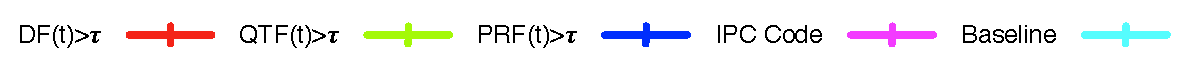
\includegraphics[width=9cm]{imgs/legend2}
\par\end{centering}

\begin{centering}
\subfigure[{Mean Average Precision.}]{\includegraphics[width=4.5cm]{imgs/figure2-MAP}}\subfigure[Recall.]{\includegraphics[width=4.5cm]{imgs/figure2-Recall}}
\par\end{centering}

\protect\caption{System performance vs. the threshold $\tau$ for four query reduction approaches.}
\label{fig:queryreduc}
\end{figure}
%%%%%%%%%%%%%%%%%%%%%%%%%%%%%%%%%%%%%%%%%%%%%%%%%%%%%%%%%%%%

%%%%%%%%%%%%%%%%%%%%%%%%%%%%%%%%%%%%%%%%%%%%%%%%%%%%%%%%%%%%
\begin{figure}[t!]
\begin{framed}
\vspace*{-2ex}
  \centering
    %\lstinputlisting[frame=single, basicstyle=\scriptsize\ttfamily , linewidth=\columnwidth,breaklines=true]{code/anecdotale.tex}\vspace*{-2ex}
 \begin{lstlisting}[basicstyle=\scriptsize\ttfamily , linewidth=\columnwidth,breaklines=true] 
PAC-1293
Abstract: The invention relates to an emulsifier, 
a method for preparing said emulsifier, and to 
its use in various applications, primarily food 
and cosmetic applications. The invention also 
relates to the use of said emulsifier for the 
creation of an elastic, gelled foam. An 
emulsifier according to the invention is based on 
a starch which is enzymatically converted, using 
a specific type of enzyme, and modified in a 
specific esterification reaction.

DF Terms: <@\textcolor{blue}{starch:14.64}@>, <@\textcolor{blue}{enzym:29.49}@>, <@\textcolor{red}{amylos:-20.15}@>, 
<@\textcolor{blue}{oil:8.63}@>, <@\textcolor{red}{dispers:-8.66}@>, <@\textcolor{red}{ph:-4.55}@>, <@\textcolor{red}{dry:-6.21}@>, <@\textcolor{red}{heat:-2.26}@>, 
<@\textcolor{red}{product:-5.48}@>, <@\textcolor{red}{slurri:-11.48}@>, <@\textcolor{blue}{viscos:7.77}@>, <@\textcolor{red}{composit:-4.49}@>, 
<@\textcolor{red}{reaction:-1.97}@>, <@\textcolor{red}{food:-11.94}@>, <@\textcolor{blue}{agent:5.19}@>, <@\textcolor{red}{debranch:-10.58}@>, 
<@\textcolor{red}{reduc:-6.37}@>, <@\textcolor{red}{fat:-12.83}@>, <@\textcolor{red}{prepar:-0.82}@>, <@\textcolor{red}{hour:-5.42}@>, 
<@\textcolor{blue}{waxi:19.41}@>, <@\textcolor{blue}{deriv:11.97}@>, <@\textcolor{red}{content:-3.38}@>, <@\textcolor{blue}{aqueou:0.38}@>, 
<@\textcolor{red}{saccharid:-11.95}@>, <@\textcolor{red}{ml:-0.79}@>, <@\textcolor{red}{cook:-10.04}@>, <@\textcolor{blue}{modifi:5.65}@>, 
<@\textcolor{blue}{solid:5.50}@>, <@\textcolor{blue}{sampl:6.27}@>, <@\textcolor{blue}{mix:2.48}@>, <@\textcolor{red}{minut:-1.68}@>, <@\textcolor{red}{dri:-0.91}@>, 
<@\textcolor{red}{gel:-9.85}@>, <@\textcolor{blue}{activ:5.98}@>, <@\textcolor{red}{corn:-5.27}@>, <@\textcolor{blue}{alpha:12}@>, <@\textcolor{red}{sprai:-2.74}@> 

QTF Terms: <@\textcolor{blue}{starch:14.64}@>, <@\textcolor{blue}{emulsifi:6.72}@>, <@\textcolor{red}{succin:-3.46}@>, 
<@\textcolor{blue}{enzym:29.49}@>, <@\textcolor{blue}{emuls:12.66}@>, <@\textcolor{blue}{hydrophob:5.45}@>, <@\textcolor{red}{anhydrid:-5.47}@>, 
<@\textcolor{red}{reaction:-1.97}@>, <@\textcolor{red}{octenyl:-0.66}@>, <@\textcolor{blue}{stabil:3.64}@>, <@\textcolor{blue}{alkenyl:0.06}@>, 
<@\textcolor{blue}{reagent:1.17}@>, <@\textcolor{blue}{carbon:0.12}@>, <@\textcolor{blue}{potato:3.74}@>, <@\textcolor{red}{alkyl:-0.33}@>, 
<@\textcolor{red}{wt:-4.57}@>, <@\textcolor{blue}{ether:1.96}@>, <@\textcolor{red}{enzymat:-3.45}@>, <@\textcolor{blue}{convers:10.44}@>, 
<@\textcolor{red}{chain:-5.53}@>, <@\textcolor{blue}{atom:0.03}@>, <@\textcolor{red}{ph:-4.55}@>, <@\textcolor{red}{treat:-0.89}@>, 
<@\textcolor{red}{ammonium:-1.96}@>, <@\textcolor{red}{food:-11.94}@>, <@\textcolor{red}{amylos:-20.15}@>, 
<@\textcolor{red}{glucanotransferas:-0.86}@>, <@\textcolor{red}{glycidyl:-0.40}@>, <@\textcolor{red}{glycosyl:-0.02}@>, 
<@\textcolor{red}{dry:-6.21}@>, <@\textcolor{blue}{deriv:11.97}@>, <@\textcolor{blue}{transferas:0.89}@>, <@\textcolor{red}{foam:-0.49}@>, 

PRF Terms: <@\textcolor{blue}{starch:14.64}@>, <@\textcolor{blue}{encapsul:17.50}@>, <@\textcolor{red}{chees:-4.22}@>, 
<@\textcolor{blue}{oil:8.63}@>, <@\textcolor{blue}{hydrophob:5.45}@>, <@\textcolor{blue}{agent:5.19}@>, <@\textcolor{red}{casein:-2.19}@>, 
<@\textcolor{blue}{degrad:17.13}@>, <@\textcolor{blue}{deriv:11.97}@>, <@\textcolor{blue}{tablet:5.30}@>, <@\textcolor{red}{debranch:-10.58}@>, 
<@\textcolor{red}{imit:-1.13}@>, <@\textcolor{blue}{viscos:7.77}@>, <@\textcolor{blue}{oxid:5.97}@>, <@\textcolor{blue}{activ:5.98}@>, <@\textcolor{blue}{osa:9.32}@>, 
<@\textcolor{blue}{funnel:2.68}@>, <@\textcolor{blue}{amylas:26.06}@>, <@\textcolor{red}{amylopectin:-7.14}@>, <@\textcolor{blue}{maiz:20.61}@>, 
<@\textcolor{red}{blend:-3.17}@>, <@\textcolor{blue}{waxi:19.41}@>, <@\textcolor{blue}{convert:31.81}@>, 

IPC title Terms:<@\textcolor{blue}{cosmet:3.77}@>, <@\textcolor{blue}{toilet:0.18}@>, <@\textcolor{red}{prepar:-0.82}@>, 
<@\textcolor{blue}{case:0.47}@>, <@\textcolor{red}{accessori:-0.01}@>, <@\textcolor{red}{store:-0.37}@>, <@\textcolor{blue}{handl:0.07}@>, 
<@\textcolor{red}{pasti:-0.17}@>, <@\textcolor{red}{substanc:-1.21}@>, <@\textcolor{red}{fibrou:-0.01}@>, <@\textcolor{red}{pulp:-1.28}@>, 
<@\textcolor{red}{constitut:-0.06}@>, <@\textcolor{blue}{paper:1.26}@>, <@\textcolor{red}{impregn:-0.11}@>, <@\textcolor{blue}{emulsifi:6.72}@>, 
<@\textcolor{red}{wet:-0.28}@>, <@\textcolor{red}{dispers:-8.66}@>, <@\textcolor{red}{foam:-0.49}@>, <@\textcolor{red}{produc:-0.57}@>, 
<@\textcolor{blue}{agent:5.19}@>, <@\textcolor{blue}{relev:0.18}@>, <@\textcolor{blue}{class:0.053}@>, <@\textcolor{red}{lubric:-0.38}@>, 
<@\textcolor{blue}{emuls:12.66}@>, <@\textcolor{red}{fuel:-0.011}@>, <@\textcolor{blue}{deriv:11.97}@>, <@\textcolor{blue}{starch:14.64}@>, 
<@\textcolor{red}{amylos:-20.15}@>, <@\textcolor{red}{compound:-0.63}@>, <@\textcolor{red}{saccharid:-11.95}@>, 
<@\textcolor{blue}{radic:1.03}@>, <@\textcolor{red}{acid:-3.19}@> 
 \end{lstlisting} 
 \vspace*{-2ex}
\end{framed}
 \vspace*{-2ex}
  \caption{Four query reduction approaches on a sample query.  Top
    terms retained by each method are shown.  Numerical oracular
    scores $\mathit{RF}(t,Q)$ are provided indicating whether the term
    was useful (blue/positive) or noisy (red/negative).}
  \label{fig:anecdotal}  
\end{figure}
%%%%%%%%%%%%%%%%%%%%%%%%%%%%%%%%%%%%%%%%%%%%%%%%%%%%%%%%%%%%

Our sample analysis of specific queries and terms selected via our oracular
approach suggests that automated methods fall far short of optimal term selection.
This leads us to explore another approach of approximating the oracular query
derived from relevance judgements by using a subset of relevance judgements
through interactive methods.  Specifically, to minimize the need for user interaction,
in this section we analyse the performance of an oracular query derived from
only the first relevant document identified in the search results.
\begin{comment}
All our attempts to improve the system effectiveness without accessing the relevance feedback were quite in vein because the features we recognized were tightly the combination of the useful words and noisy words and the system performance is too sensitive to the existence of a noisy word or the absence of the useful terms. So, we decided to apply much more realistic approach in which feedback terms are extracted only from the first ranked relevant document retrieved. 
\end{comment}
Using this approach, Table \ref{tab:firstrel} shows that we can double the MAP in comparison to our baseline and also outperform the PATATRAS system.

%%%%%%%%%%%%%%%%%%%%%%%%%%%%%%%%%%%%%%%%%%%%%%%%%%%%%%%%%%%%%%%%
\begin{table}[t!]
  \begin{center}
   \caption{System performance using minimal relevance feedback. $\tau$ is RF score threshold, and $k$ indicates the number of first relevant retrieved patents.}\vspace{3mm}
  \input table/partialRFtermselect.tex   
  \label{tab:firstrel}
  \end{center}  
\end{table}
%%%%%%%%%%%%%%%%%%%%%%%%%%%%%%%%%%%%%%%%%%%%%%%%%%%%%%%%%%%%%%%%

Furthermore, to establish the minimal interaction required by this
approach, Figure \ref{fig:FirstTPRankHisto} indicates that the
baseline methods return a relevant patent approximately 80\% of the
time in the first 10 results and 90\% of the time in the first 20
results.  Hence, such an interactive approach requires relatively low
user effort while achieving state-of-the-art performance.


\begin{figure}
\begin{centering}
\includegraphics[width=5.5cm]{imgs/1stRank}
\par\end{centering}

\protect\caption{The distribution of the first relevant document rank over test queries.}
\label{fig:FirstTPRankHisto}
\end{figure}




\section{Related Work}
\label{Sec:RelatedWork}
% Reda: please have a look at this section and consider revising
%       as appropriate.  -Scott


Our work is different from pioneer studies on patent retrieval, as we
closely looked into the problem rather than solutions to figure out
the causes that generic IR models which are based on term matching
process, do not work efficiently in patent domain. However, we cite here few works that focus mainly on query reformulation for patent search. 
In \cite{Itoh2003}, authors proposed a new term selection method using different term
frequencies depending on the genre in the NTCIR-3 Patent Retrieval Task.
Xue and Croft \cite{xue2009transforming} conducted a series of experiments
in order to examine the effect of different patent fields, and concludes
with the observation that the best MAP is
achieved using the text from the description section. Also, Fuji \cite{Fujii2007}
showed that retrieval effectiveness can be improved by combining IR
methods with the result of citation extraction.
Bashir et al. \cite{Bashir2010} propose query expansion with pseudo-relevance
feedback. Terms are selected using a using a machine
learning approach, by picking terms that may have a potential positive
impact on the retrieval effectiveness. Verma and Varma
\cite{Verma2011} propose a different approach, which instead of using
the patent text to query, use its IPC codes, which are expanded using the citation network. The formed
query is used to perform an initial search. The results are then re-ranked
using queries constructed from patent text.
Magdy et al.~\cite{magdy2011study} studied works on query expansion in patent
retrieval and discussed that standard query expansion techniques are
less effective, where the initial query is the full texts of query
patents. Mahdabi et al.~\cite{Mahdabi2013} used term proximity
information to identify expansion terms. Ganguly et
al.~\cite{ganguly2011patent} adapted pseudo relevance feedback for
query reduction by decomposing a patent application into constituent
text segments and computing the Language Modelling (LM) similarities
of each segment from the top ranked documents. The least similar
segments to the pseudo-relevant documents removed from the query,
hypothesizing it can increase the precision of retrieval. Kim et
al.~\cite{kim2014diversifying} provided diverse query suggestion using
aspect identification from a patent query to increase the chance of
retrieving relevant documents. Mahdabi et al.~\cite{mahdabi2014patent}
used linked-based structure of the citation graph together with IPC
classification to improve the initial patent query. 
Finally, other works investigated query suggestion for patent prior
art search, which reflect real-life scenario of examiners, who form
reproducible boolean queries \cite{Adams2011,Azzopardi2010,Kim2011}.



% A ``Conclusion'' is not entirely necessary in a poster paper...
% include only if there is sufficient space.  -Scott
%
\section{Conclusion}
\label{Sec:Conclusion}
\chapter{Conclusions}
\label{cha:conc}
%\textcolor{red}{Mona: I will compose this chapter after we confirmed about all chapters!}\\
%Summary your thesis and discuss what you are going to do in the future in Section~\ref{sec:future}.

%\section{Overview}
%\label{sec:overview}
\section{Summary}
\label{sec:summary}

In this thesis, we investigated the reasons that patent prior art searches 
are less effective than the other web search applications on CLEF-IP 2010 data collection. 
We started with recognizing errors due to data curation and baseline settings that 
make small portions of the whole retrieval errors. The main portion of the errors are 
due to term matching process in retrieval ranking functions. 
Hence, we looked at the patent prior art search from
a term selection perspective. While previous works proposed
different solutions to improve retrieval effectiveness, we 
focused on term analysis of the patent query and top-100 retrieved patents. 
After defining an oracular query based on
relevance judgements, we established both the sufficiency
of the standard LM retrieval scoring models and query reduction 
methods to achieve state-of-the-art patent prior art
search performance. After finding that automated methods 
for query reduction approaches fail to offer significant
performance improvements, we showed that we can double
the MAP with minimum user interaction by approximating
the oracular query through a relevance feedback approach
with a single relevant document. Given that such simple 
interactive methods for query reduction with a standard LM
retrieval model outperform highly engineered patent-specific
search systems from CLEF-IP 2010, we concluded that interactive 
methods offer a promising avenue for simple but
highly effective term selection in patent prior art search.
 

\section{Contributions}
\label{sec:contributions}
We briefly summarize the major contributions of our work as follows:
\begin{enumerate}
\item \textbf{Oracular term selection system: }We built an oracular term selection system from known relevance judgments to formulate an oracular query that far outperformed the baseline and the best-performed competitor on CLEF-IP 2010 which made the following points clear for us:
\begin{enumerate}
\item We calculated an oracular score to recognize the positive terms and the negative terms;
\item We observed the disruptive effect of including negative terms in queries;
\item We noticed the sufficiency of terms in the reference patent query; and 
\item We concluded that query reduction and precise query term selection methods suffice for an effective prior art patent retrieval.
\end{enumerate}
\item \textbf{Automated query reduction: } We examined four simple query reduction methods to select the positive terms and prone out the negative terms. We illustrated that these approaches are inefficient because they can not discriminate between useful and noisy words. Since our system is over-sensitive to the existence of noisy words, we could not achieve high performance via these simple methods. 
\item \textbf{Proposing a semi-interactive method for query term selection: }We showed that a simple minimal interactive relevance feedback approach where terms are selected by only the first retrieved relevant document performs as well as a highly engineered patent-specific system on CLEF-IP 2010. 
\end{enumerate}

\section{Future Work}
\label{sec:future}






%ACKNOWLEDGMENTS are optional
%\section{Acknowledgments}
%NICTA is funded by the Australian Government as represented by the Department of Broadband, Communications and the Digital Economy and the Australian Research Council through the ICT Centre of Excellence program.

% The following two commands are all you need in the
% initial runs of your .tex file to
% produce the bibliography for the citations in your paper.
\bibliographystyle{abbrv}
{\scriptsize
\bibliography{sigproc}
} % sigproc.bib is the name of the Bibliography in this case
% You must have a proper ".bib" file
%  and remember to run:
% latex bibtex latex latex
% to resolve all references
%
% ACM needs 'a single self-contained file'!
%
%APPENDICES are optional
%\balancecolumns
%\appendix
%%Appendix A
%\section{Headings in Appendices}
%The rules about hierarchical headings discussed above for
%the body of the article are different in the appendices.
%In the \textbf{appendix} environment, the command
%\textbf{section} is used to
%indicate the start of each Appendix, with alphabetic order
%designation (i.e. the first is A, the second B, etc.) and
%a title (if you include one).  So, if you need
%hierarchical structure
%\textit{within} an Appendix, start with \textbf{subsection} as the
%highest level. Here is an outline of the body of this
%document in Appendix-appropriate form:
%\subsection{Introduction}
%\subsection{The Body of the Paper}
%\subsubsection{Type Changes and  Special Characters}
%\subsubsection{Math Equations}
%\paragraph{Inline (In-text) Equations}
%\paragraph{Display Equations}
%\subsubsection{Citations}
%\subsubsection{Tables}
%\subsubsection{Figures}
%\subsubsection{Theorem-like Constructs}
%\subsubsection*{A Caveat for the \TeX\ Expert}
%\subsection{Conclusions}
%\subsection{Acknowledgments}
%\subsection{Additional Authors}
%This section is inserted by \LaTeX; you do not insert it.
%You just add the names and information in the
%\texttt{{\char'134}additionalauthors} command at the start
%of the document.
%\subsection{References}
%Generated by bibtex from your ~.bib file.  Run latex,
%then bibtex, then latex twice (to resolve references)
%to create the ~.bbl file.  Insert that ~.bbl file into
%the .tex source file and comment out
%the command \texttt{{\char'134}thebibliography}.
%% This next section command marks the start of
%% Appendix B, and does not continue the present hierarchy
%\section{More Help for the Hardy}
%The sig-alternate.cls file itself is chock-full of succinct
%and helpful comments.  If you consider yourself a moderately
%experienced to expert user of \LaTeX, you may find reading
%it useful but please remember not to change it.
%\balancecolumns % GM June 2007
% That's all folks!



\end{document}
